\documentclass[journal]{IEEEtran}
\usepackage[a5paper, margin=10mm, onecolumn]{geometry}
\usepackage[cmex10]{amsmath}
\usepackage{amssymb,amsfonts,amsthm}
\usepackage{gvv-book}
\usepackage{gvv}
\usepackage{hyperref}


\begin{document}
\title{5.8.23}
\author{EE25BTECH11025 - Ganachari Vishwambhar}
\maketitle

\textbf{Question}:\\
A lending library has a fixed charge for the first three days and an additional charge for each day thereafter. Sarita paid 27 rupees for seven days, while Susheela paid 21 rupees for five days. Find the fixed charge and the charge for each extra day.\\
\textbf{Solution: }\\
Let:\\
The cost for the first three days be $x$.\\
The additional cost be $y$.\\
Given:
\begin{align}
    \myvec{3&4}\myvec{x\\y} = 27\\
    \myvec{3&2}\myvec{x\\y} = 21
\end{align}

Solving (1) and (2):
\begin{align}
    \augvec{2}{1}{3&4&27\\3&2&21}R_2\rightarrow R_2-R_1\\
    \augvec{2}{1}{3&4&27\\0&-2&-6}R_1\rightarrow R_1+2R_2\\
    \augvec{2}{1}{3&0&15\\0&-2&-6}R_1\rightarrow \frac{1}{3}R_1;R_2\rightarrow \frac{-1}{2}R_2\\
    \augvec{2}{1}{1&0&5\\0&1&3}
\end{align}

The charge for the first three days is 5.\\
The additional charge is 3.

\begin{figure}[h!]
   \centering
   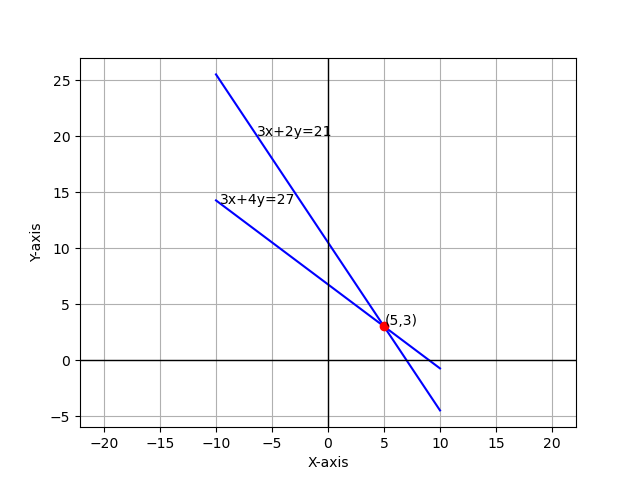
\includegraphics[width=0.7\linewidth]{figs/plot.png}
   \caption{Plot of the given system of equations}
   \label{}
\end{figure}
\end{document}
